% 再実行報告 (2026-08-18)。LuaTeX + luatexja-fontspec で日本語組版する。
% コンパイル: lualatex main.tex を 2 回。
\documentclass[11pt]{article}
\usepackage{luatexja-fontspec}
\setmainjfont[BoldFont=IPAexGothic]{IPAexMincho}
\setsansjfont{IPAexGothic}
\usepackage[margin=25mm]{geometry}
\usepackage{amsmath}
\usepackage{booktabs}
\usepackage{graphicx}
\usepackage{array}
\usepackage[hidelinks]{hyperref}
\usepackage{caption}
\captionsetup{font=small, labelfont=bf}

\title{\textbf{OpenDDE 4ノード分散ファインチューニング再実行報告}\\
{\large --- 共有リソースパスへの差し替えと前回記録との差異の検証 ---}}
\author{松澤 拓海}
\date{2026年8月18日}

\begin{document}
\maketitle

\begin{abstract}
前回の技術報告（2026-08-15、リポジトリ \texttt{matsuzawa-20260815-opendde-multinode-longrun} の paper.pdf）と同一の実験
──OpenDDE 拡散モジュールの4ノード分散ファインチューニングと実行正当性検証──を、
データパスのみ個人領域（rku00122）から共有セットアップへ差し替えて Seyval 経由で再実行した
（run\_id: \texttt{8448dcf3-1a6e-4fbf-8a34-2b3b5abdad00}、コミット \texttt{96d5076}）。
分散実行の検証は前回と同様 \textbf{PASS} し、4ノード16 GPU・全ランク合計960ステップ・
学習ループ実測時間（1412.5秒 対 前回1411秒）まで前回とほぼ一致した。
一方、学習損失の軌跡は前回と一致せず、エポック平均損失への線形回帰は今回、
名目上有意な減少（傾き $-2.47\times10^{-4}$/エポック、$p=0.021$）を示した。前回は $p=0.49$（有意でない）である。
この不一致の原因は学習コードが乱数シードを固定していないことにあり、
同一設定の3ラン（前回・再現・今回）で $p$ 値は $0.49/0.17/0.021$ と大きく散らばる。
今回の「有意」を学習進行の証拠と読むべきではなく、前回報告の
「この規模の減少は本実験の検出力では区別できない」という記述と整合するラン間変動と解釈するのが妥当である。
FoldBench 抗体--抗原評価（DockQ）は今回のチェックポイントに対しては未実施である。
\end{abstract}

\section{実行構成 --- 前回からの変更点はパスのみ}

コード・ハイパーパラメータ・ノード数（\texttt{expect\_nodes: 4}）は前回のまま変更していない。
変更したのは rku00122 個人領域を指していたパスのみで、いずれも共有セットアップの同等物へ差し替えた
（表~\ref{tab:paths}）。実行は Seyval の BYO Slurm クラスタ「RIKYU」上で、
4ノード $\times$ NVIDIA GB200 4基 $=$ 16 GPU（1 GPU 1プロセス、aarch64）を占有し、
コミット済み Dockerfile から構築したイメージで行った。

\begin{table}[h]
\centering
\caption{パス差し替えの内容（\texttt{config/run/proposed-opendde-openfold3.yaml} および \texttt{docker/Dockerfile.eval}）。
以下 \texttt{\$SHARED} $=$ \texttt{/data1/rkp00041/plinder\_lddt\_pli\_improvement}。}
\label{tab:paths}
\small
\begin{tabular}{@{}p{0.38\linewidth}p{0.56\linewidth}@{}}
\toprule
項目 & 差し替え後 \\
\midrule
\texttt{opendde\_root} & \texttt{\$SHARED/model/opendde\_data} \\
\texttt{checkpoint}（事前学習済み） & \texttt{\$SHARED/model/opendde\_data/checkpoint/opendde.pt} \\
\texttt{python\_bin} & \texttt{\$SHARED/model/opendde/.venv/bin/python}（共有 venv） \\
\texttt{cache\_dir}（学習データ） & \texttt{/data1/rkp00041/rku00121/mz-repro-cache/sft}（武藤氏が同一スクリプトで共有データから再生成した30件） \\
Dockerfile.eval の微調整済み CKPT 参照 & 武藤氏再現ランの \texttt{finetuned.pt}（今回のランの成果物ではない。\S\ref{sec:eval} 参照） \\
\bottomrule
\end{tabular}
\end{table}

\section{分散実行の検証 --- 前回と同水準で PASS}
\label{sec:validation}

検証機構（全ランクがホスト名と GPU UUID を報告し、集団通信で集約する方式）の集約結果を
表~\ref{tab:placement} に示す。物理ノードは前回と異なるが、並列度・ステップ数・学習ループ実測時間は一致しており、
計算の量と構造は前回と同一である。

\begin{table}[h]
\centering
\caption{分散実行の集約結果の比較。}
\label{tab:placement}
\small
\begin{tabular}{@{}lll@{}}
\toprule
項目 & 前回（2026-08-15） & 今回（2026-08-18） \\
\midrule
相異なるホスト数 & 4（c050, c054, c055, c056） & 4（c180, c182, c185, c186） \\
ホストごとのランク数 / 相異なる GPU UUID & 各4 / 16 & 各4 / 16 \\
全ランク合計ステップ（ランクあたり） & 960（60） & 960（60） \\
学習ループ実行時間 & 1411秒 & 1412.5秒 \\
ジョブ全体 & 2459秒 & 1666秒 \\
判定 & PASS & PASS \\
\bottomrule
\end{tabular}
\end{table}

ジョブ全体の793秒の短縮は、実行イメージの準備とデータ読み込みの差であり、学習そのものの速度差ではない。
学習対象データも前回と同一であることをログから確認した：27エントリの PDB ID 集合が一致し、
「22件が各エポック1回・5件が2回」という16ランクへの割り付けパターン（27標本 $\to$ 32スロット）も
前回報告の記載どおりであった。原子数4{,}000超で除外された3件（5f8q, 5w41, 6ejd）も同一である。
なお前回報告にあった負の対照実験（1ノードで4ノードを要求して FAIL させる）は今回は再実施していない。

\section{学習損失 --- 軌跡は前回と一致しない}
\label{sec:loss}

図~\ref{fig:loss} にエポック平均損失の推移を、表~\ref{tab:loss} に同一設定3ランの統計を示す。
今回のランに限れば、回帰は名目上有意な減少を示す
（$t(28)=-2.45$、$p=0.021$、傾きの95\%信頼区間 $[-4.5\times10^{-4},\,-0.4\times10^{-4}]$）。
30エポックでの累積減少は点推定で約0.0072に相当し、これは前回報告が
「信頼区間の下端（0.0077の減少）に相当する変動があっても本実験の検出力では区別がつかない」と述べた、
まさにその規模である。

\begin{figure}[h]
\centering
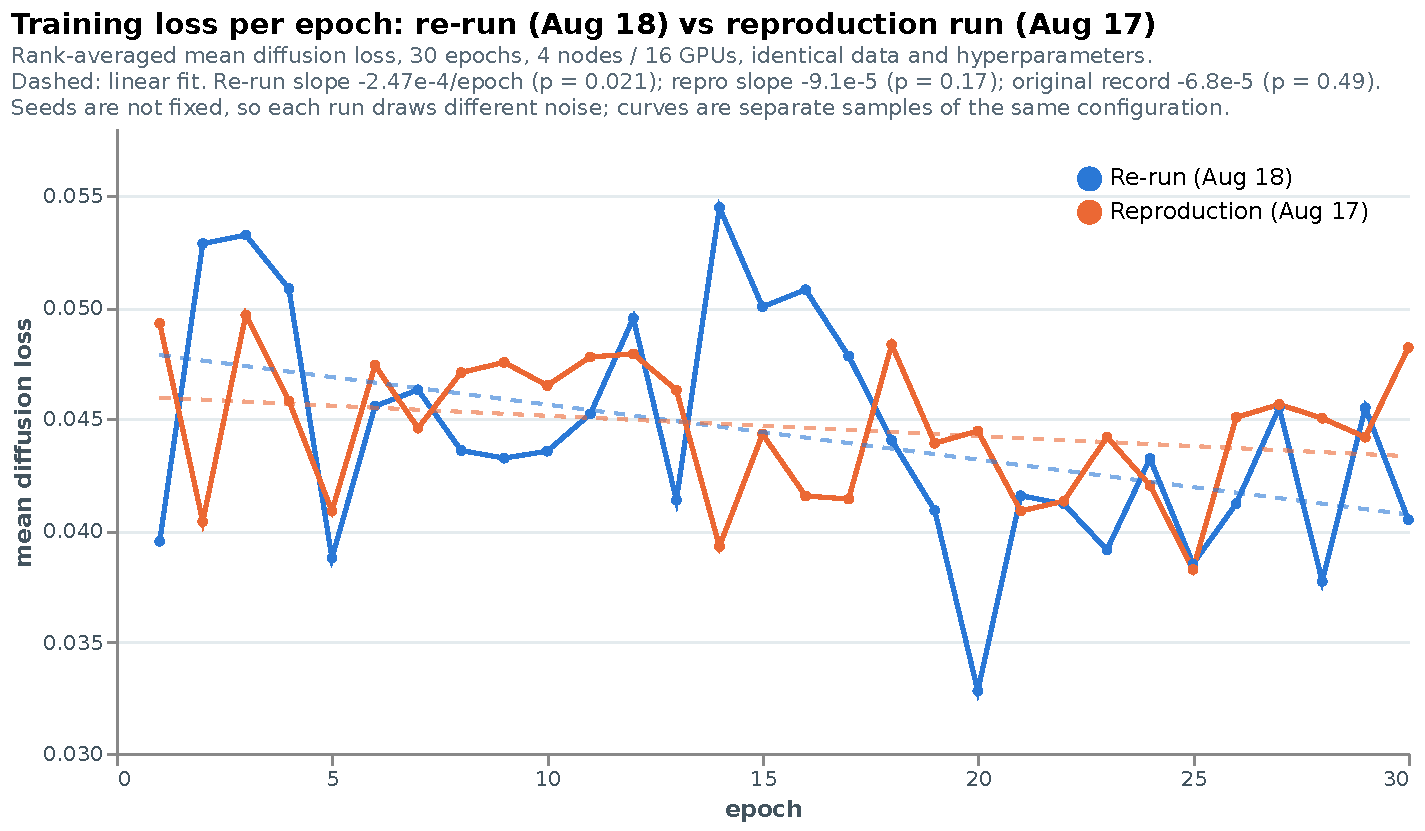
\includegraphics[width=0.95\linewidth]{../../results/chart/loss_rerun_comparison.pdf}
\caption{エポック平均の拡散損失（30エポック、全ランク平均）。青が今回（08-18）、橙が武藤氏再現ラン（08-17）、破線は線形回帰。
縦軸は0.030--0.057に拡大している（ゼロ起点ではない）。前回報告（08-15）の生データは未入手のため要約統計のみ表~\ref{tab:loss}に示す。}
\label{fig:loss}
\end{figure}

\begin{table}[h]
\centering
\caption{同一設定3ランの学習損失統計。「開始$\to$終了」は各ランクのステップ前半1/4と後半1/4の平均
（検証機構の loss\_start / loss\_end）。$^{*}$前回報告の値は初回/最終エポックの平均として記載されていたもので、定義が異なる。
回帰はエポック番号に対する単回帰（$n=30$, $\mathrm{df}=28$）、$p$ 値は両側 $t$ 検定。}
\label{tab:loss}
\small
\begin{tabular}{@{}lcccccc@{}}
\toprule
ラン & 平均 & 範囲 & 開始$\to$終了 & 傾き /エポック & $r^2$ & $p$ 値 \\
\midrule
前回報告（08-15） & --- & 0.0373--0.0556 & 0.0498$\to$0.0469$^{*}$ & $-6.8\times10^{-5}$ & 0.018 & 0.49 \\
武藤氏再現（08-17） & 0.0446 & 0.0383--0.0497 & --- & $-9.1\times10^{-5}$ & 0.066 & 0.17 \\
今回（08-18） & 0.0443 & 0.0328--0.0545 & 0.0467$\to$0.0415 & $-2.47\times10^{-4}$ & 0.176 & \textbf{0.021} \\
\bottomrule
\end{tabular}
\end{table}

\section{なぜ前回と結果が異なるのか}
\label{sec:why}

計算内容が同一（\S\ref{sec:validation}）であるにもかかわらず損失の軌跡と検定結果が異なる理由は、
消去法で明確に特定できる。

\subsection{主因：乱数シードが固定されていない}

\texttt{src/train.py} には \texttt{torch.manual\_seed} の呼び出しが存在しない。
拡散学習の各ステップでは、ノイズ強度 $\sigma$ の対数正規サンプリング
（\texttt{sample\_noise\_level} 内の \texttt{torch.randn}）と、座標への付加ノイズ
（\texttt{torch.randn\_like}）がシードなしで描画される。
EDM 損失は $\sigma$ に強く依存する（$\sigma$ が大きいステップほど課題が難しい）ため、
1エポックあたり全ランク合計32ステップ $\times$ 4ノイズ標本という標本数では、
$\sigma$ の引きの偏りだけでエポック平均が大きく揺らぐ。
つまり各ランの損失曲線は同じ分布からの別の標本であり、一致しないのが正常である。

\subsection{帰結：回帰の「有意性」はラン間で再現しない}

同一設定の3ランで $p$ 値は $0.49 \to 0.17 \to 0.021$ と揺れ、傾きの点推定も
$-6.8\times10^{-5}$ から $-2.47\times10^{-4}$ まで3.6倍の幅で動いた。
今回の $p=0.021$ だけを取り出して「30エポックで学習が進むようになった」と解釈するのは誤りで、
3ラン全体は「微小な減少傾向はあるかもしれないが、単一ランの検出力では確定できない」という
前回報告の結論の範囲内にある。傾きの符号が3ランとも負である点は減少傾向の存在を弱く支持するが、
確証には複数シードでの反復か、より長い学習が必要である。

\subsection{差し替えたデータパスは原因ではない}

学習キャッシュは武藤氏が同一の前処理スクリプトで同一の共有データ
（OpenFold3 PDB サブセット）から再生成したものであり、
エントリ選定規則（解像度昇順の先頭30件）は決定的である。
実際、今回学習に使われた27件の PDB ID・除外3件・重複割り付けパターンは前回の記載と完全に一致した
（\S\ref{sec:validation}）。物理ノードの違い（c050系 $\to$ c180系）も、
GPU 個体差や非決定的 CUDA カーネルの丸め差はシード非固定による変動に比べ桁違いに小さく、
観測された差の説明にはならない。

\paragraph{再現性への提言}
次回以降このランを比較の基準に使うなら、\texttt{src/train.py} の学習開始時に
ランク固有のシード（例：\texttt{torch.manual\_seed(base\_seed + rank)}）を固定すべきである。
固定すれば同一ハード・同一データでの損失曲線は（非決定的カーネルの丸めを除き）一致し、
「差が出たらコードの変化を疑える」状態になる。現状は差が出てもシードの引き直しと区別できない。

\section{DockQ 評価の状況 --- 今回のチェックポイントでは未実施}
\label{sec:eval}

本ランの成果物 \texttt{finetuned.pt} に対する FoldBench 抗体--抗原評価はまだ実行していない。
参考として、既存の2つの評価結果を表~\ref{tab:dockq} に併記する。
両者は評価対象セットが異なるため直接比較できない
（前回報告は16ターゲットから原子数で2件除外した14ターゲット19インターフェース、
武藤氏再現は上限20ターゲット設定で26試行・24採点）。

\begin{table}[h]
\centering
\caption{既存評価の参考値（MSA・テンプレート検索なし）。いずれも今回のチェックポイントの評価ではない。}
\label{tab:dockq}
\small
\begin{tabular}{@{}lcccc@{}}
\toprule
評価 & 成功率（事前学習） & 成功率（微調整後） & DockQ 平均 & lDDT 平均 \\
\midrule
前回報告（19 IF、Wilcoxon $p=0.16$） & 10.53\% & 10.53\% & 0.0844$\to$0.0693 & 0.660$\to$0.643 \\
武藤氏再現（24採点） & 8.33\% & 12.5\% & 0.0744$\to$0.0730 & 0.679$\to$0.670 \\
\bottomrule
\end{tabular}
\end{table}

注目すべきは変化の方向が逆である点だ（前回：成功率横ばい・平均低下／再現：成功率微増・平均横ばい）。
いずれも数件のインターフェースの出入りによる差であり、
「微調整の効果は現在の評価規模ではノイズと区別できない」という前回報告の結論をむしろ補強している。
今回のチェックポイントを評価する場合は、\texttt{docker/Dockerfile.eval} の微調整済みチェックポイント参照
（現在は武藤氏再現ランの成果物を指す）を本ランの \texttt{finetuned.pt} に差し替えたうえで
eval を実行する必要がある。

\section{成果物}

本ランの成果物は Seyval 側に保存されている（RIKYU 上のジョブ作業ディレクトリは実行後に削除済み）。

\begin{itemize}
  \item \texttt{.research/results/proposed-opendde-openfold3/finetuned.pt}（2.6 GB）--- 微調整済みチェックポイント
  \item 同 \texttt{loss\_curve.json} --- エポック平均損失（図~\ref{fig:loss}・表~\ref{tab:loss} の元データ）
  \item 同 \texttt{placement.json} --- 全16ランクのホスト名・GPU UUID 記録
\end{itemize}

リポジトリへ取り込む場合は \texttt{import\_run\_outputs}、
後続ランへ渡す場合は \texttt{start\_run} の \texttt{inputs\_from\_runs} を使用する。

\vspace{2em}
\noindent\rule{\linewidth}{0.4pt}\\
{\small
作成：2026-08-18／松澤 拓海（実行・集計は Claude Code + AIRAS/Seyval MCP）。
参照：前回報告 $=$ \texttt{auto-res2/matsuzawa-20260815-opendde-multinode-longrun} の
\texttt{.research/results/paper.pdf}、再現ラン $=$ \texttt{/data1/rkp00041/rku00121/mz-repro/}。}

\end{document}
